
\documentclass[aspectratio=169]{beamer}
\usetheme{Madrid}
 
\usepackage{graphicx}
%\usepackage[spanish]{babel}
\usepackage[utf8]{inputenc}
\usepackage{hyperref}
\usepackage{verbatim}


\AtBeginSection[]
{
	\begin{frame}
		\frametitle{Table of Contents}
		\tableofcontents[currentsection]
	\end{frame}
}


\begin{document}


\title{Introduction to neural networks}  
\subtitle{Regression introduction} 
\author[J.I. Vasquez]{\textbf{Juan Irving Vásquez} \\jivg.org}
\date{\today \copyright}
\institute[jivg.org]{Centro de Innovación y Desarrollo Tecnológico en Cómputo \\ Instituto Politécnico Nacional}
% logo of my university
\titlegraphic{
\includegraphics[width=2cm]{ipn-cidetec}}
\frame{\titlepage} 

%%%%%%%%%%%%%%%%%%%%%%%%%%%%%%%%%%%%%%%%%%%%%%%%%%%%%%%%

\frame{
	\frametitle{Contents}
\tableofcontents
}



%\frame{
%	\frametitle{Deep Learning Approach}
%\begin{center}
%	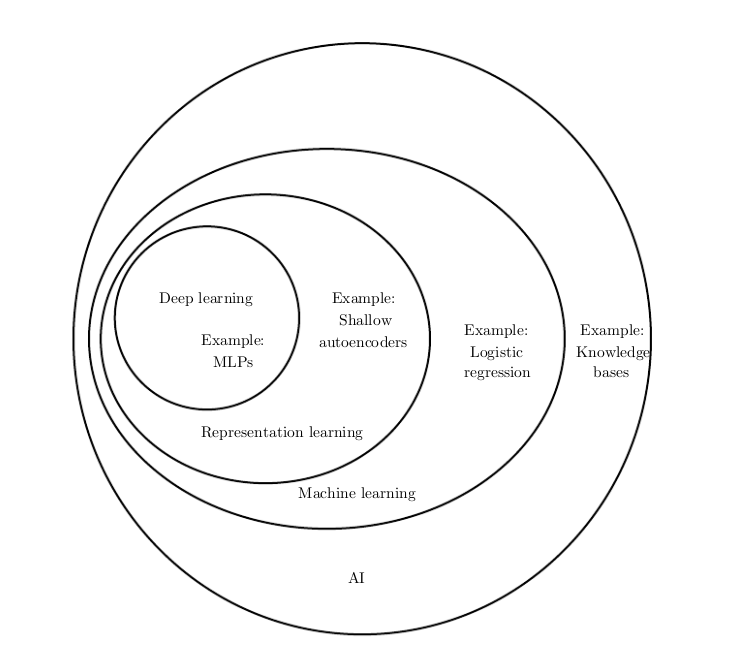
\includegraphics[width=0.7\linewidth]{venn}
%\end{center}
%}


%\frame{
%	\frametitle{Bibliography}
%	\begin{itemize}
%		\item Szeliski, R. (2010). \textit{Computer vision: algorithms and applications.} Springer Science \& Business Media.
%		\item I Goodfellow, Y Bengio, A Courville, Y. Bengio. \textit{Deep learning}. 
%		\item Pytorch \url{https://pytorch.org/}
%		\item Torchvision. \url{https://pytorch.org/docs/stable/torchvision/}
%		%\item Jain Kasturi Schunck,\textit{Machine Vision}, Mac Graw Hill.
%		%\item Scopatz, A., \& Huff, K. D. (2015). \textit{Effective computation in physics: Field guide to research with python.} O' Reilly Media, Inc.
%	\end{itemize}
%	
%	\begin{figure}
%		\centering
%		
\includegraphics[height=0.4\textheight]{szeliski}
%		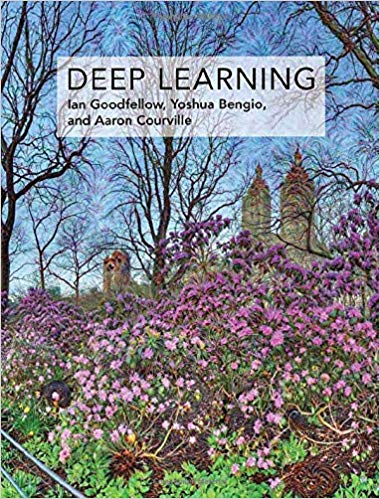
\includegraphics[height=0.4\textheight]{goodfellow}
%		%\includegraphics[width=0.2\linewidth]{jain}
%		%\includegraphics[width=0.2\linewidth]{scopatz}
%		%\caption{}
%		\label{fig:szeliski}
%	\end{figure}	
%}


%\frame{
%	\frametitle{Bibliography}
%	\begin{itemize}
%		\item Goodfellow, Ian, et al. Deep learning. Vol. 1. Cambridge: MIT press, 2016.
%		\item Walpole, R. E., Myers, R. H., Myers, S. L., \& Ye, K. Probability and statistics for engineers and scientists (9th Ed). New York: Macmillan.
%		\item Vishnu Subramanian, Deep Learning with PyTorch, 2018.
%	\end{itemize}
%}


%\frame{
%	\frametitle{Resources}
%	\begin{itemize}
%		\item Repository: 
%		\url{https://github.com/irvingvasquez/practicas_pytorch}
%		\item Slides: \\
%		\url{https://jivg.org/courses/vision-computacional/}
%	\end{itemize}
%}


\section{Linear Regression}


\frame{
\frametitle{Linear regression}
%\begin{itemize}
%\item 
%\end{itemize}

\begin{figure}
\centering
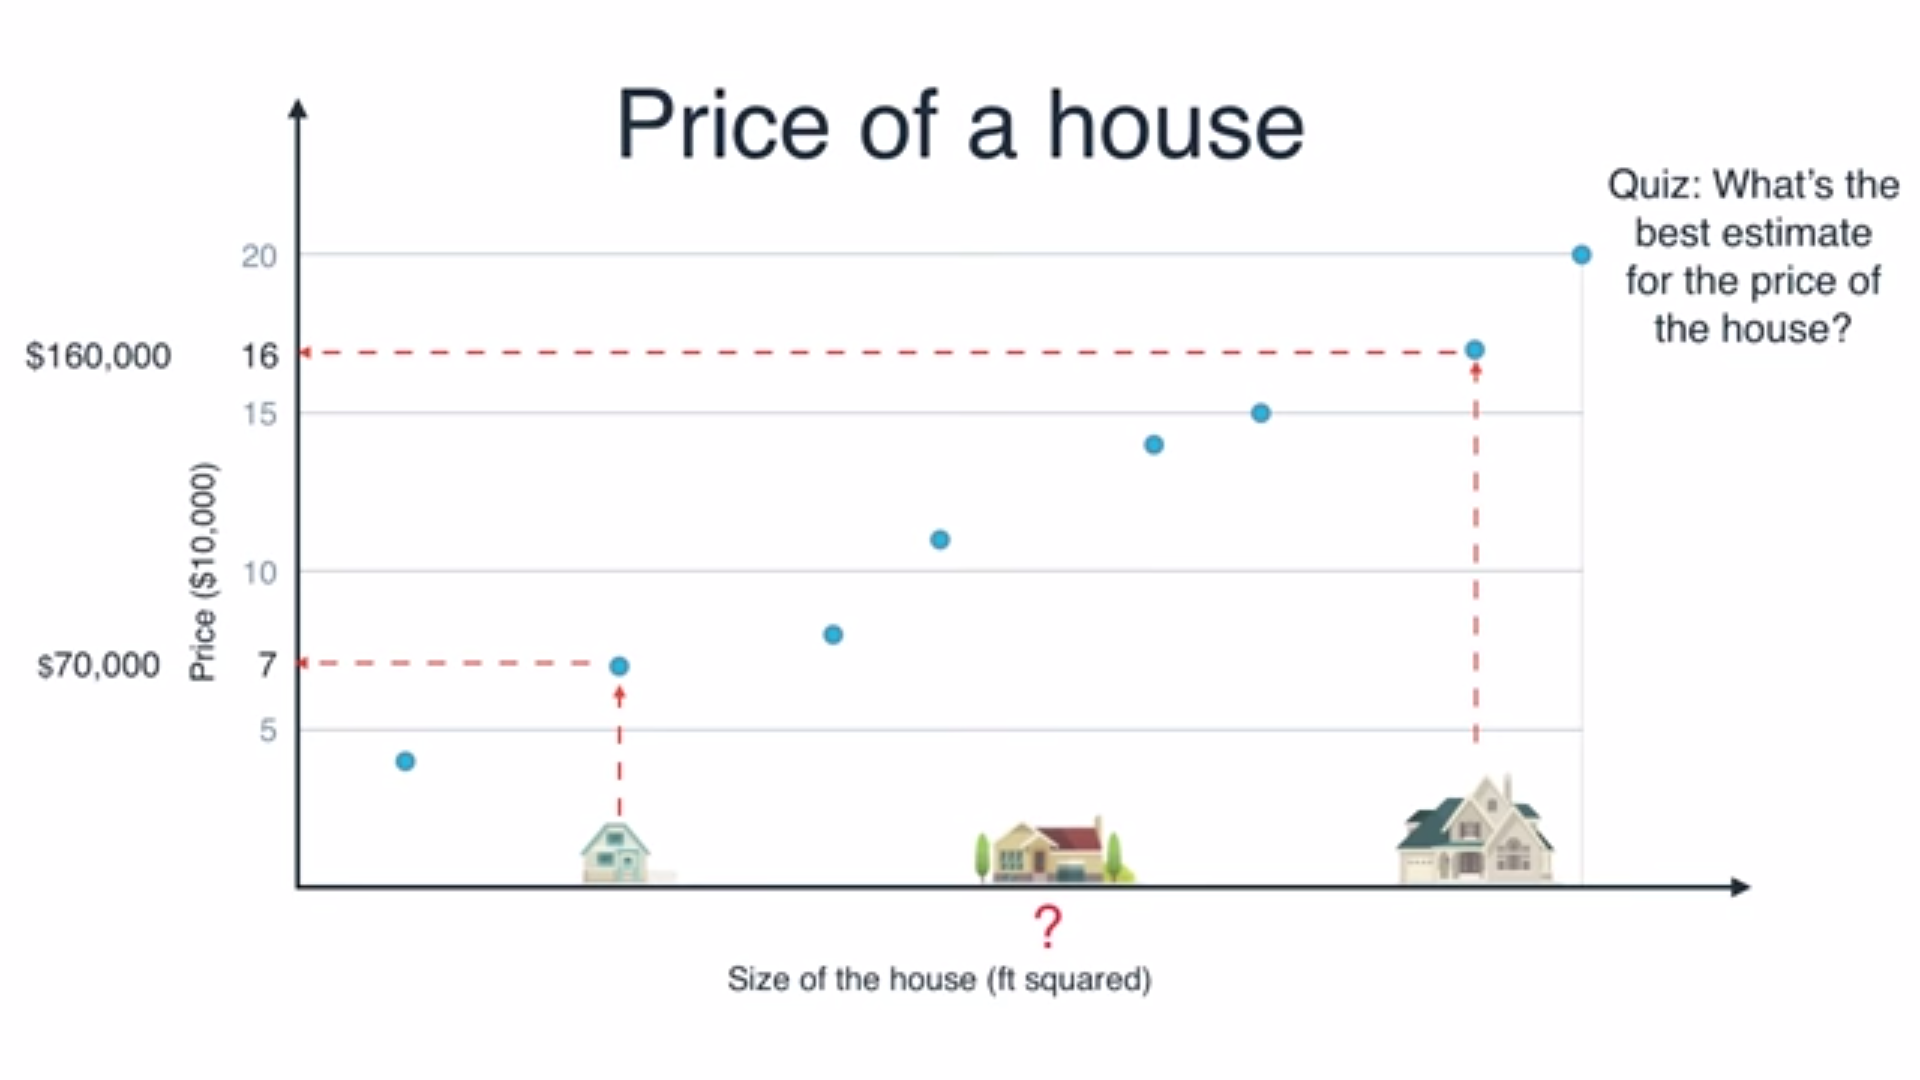
\includegraphics[height=0.8\textheight]{./inn}
%\caption{}
\label{}
\end{figure}
}


\frame{
\frametitle{Linear regression}
\begin{itemize}
\item A relation between:
\item Independent variables (regressors)
\item Dependent variables (responses)
\begin{equation}
Y = \beta_0 + \beta_1 x
\end{equation}
\item $\beta_0$ is the intercept
\item $\beta_1$ is the slope
\end{itemize}
}


\frame{
\frametitle{Linear regression}
%\begin{itemize}
%\item Deterministic
%\end{itemize}
\begin{figure}
\centering
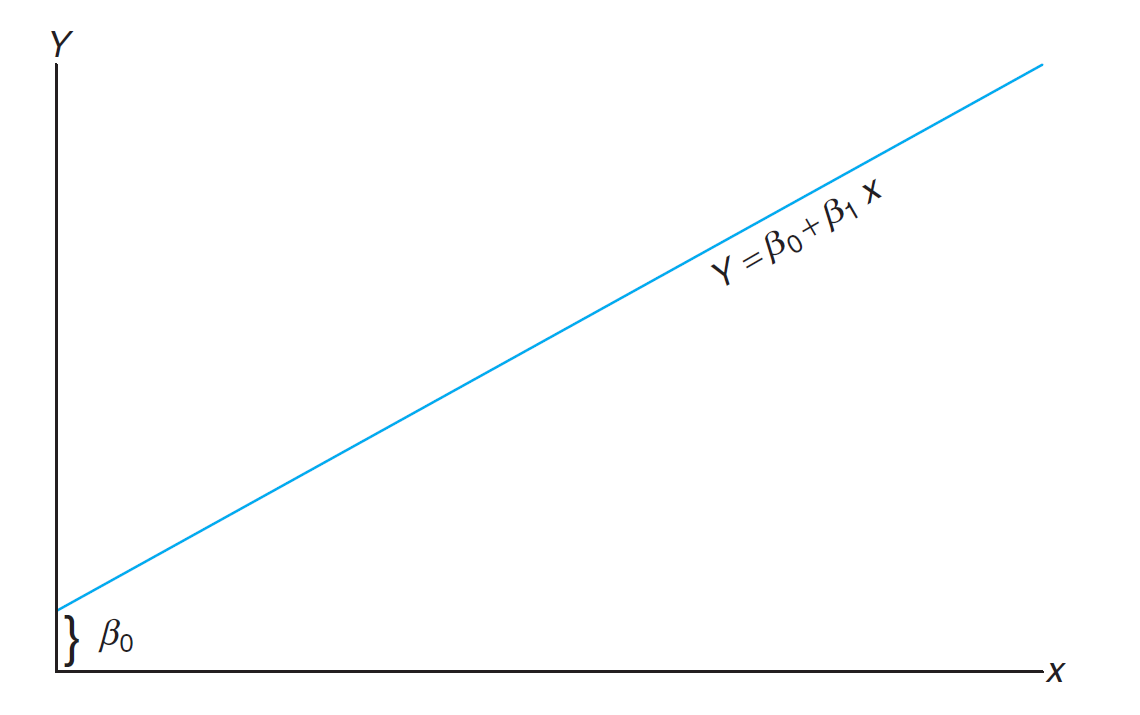
\includegraphics[height=0.7\textheight]{./lr}
\caption{Deterministic equation for a linear model}
\label{fig:lr}
\end{figure}
}


\frame{
\frametitle{Simple Linear Regression (SLR) Model}
\begin{itemize}
\item SLR Model

\begin{equation}
Y = \beta_0 + \beta_1 x + \epsilon
\end{equation}
\item where $E(\epsilon) =0$ and $Var(\epsilon) = \sigma^2$
\end{itemize}
}


\frame{
\frametitle{Simple Linear Regression (SLR) Model}
\begin{itemize}
\item What does it mean?
\begin{figure}
\centering
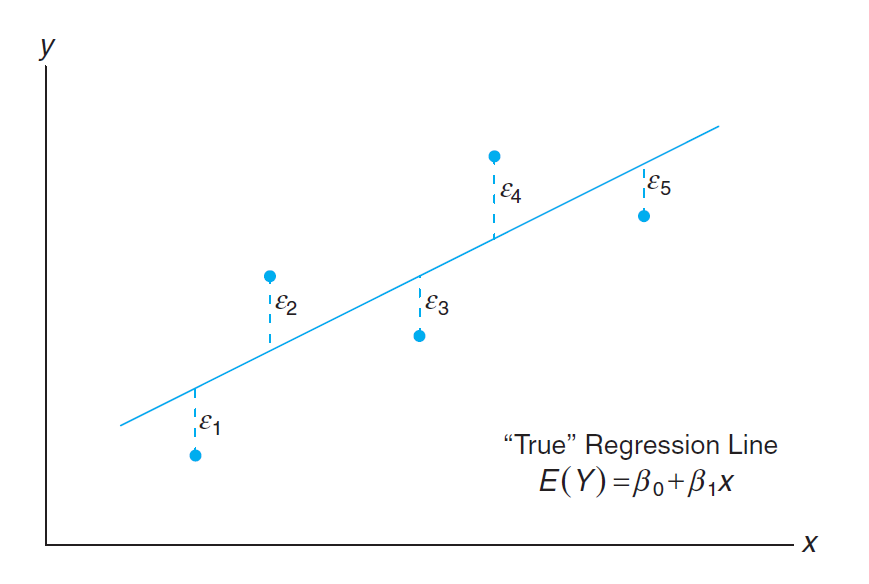
\includegraphics[height=0.7\textheight]{./lr1}
%\caption{}
\label{fig:lr1}
\end{figure}
\end{itemize}
}



\frame{
\frametitle{Fitted regression line}
\begin{itemize}
\item To estimate the regression coefficients ($\beta_0$,$\beta_1$)
\begin{equation}
\hat{y} = b_0 + b_1 x
\end{equation}
 
\end{itemize}
}



\frame{
\frametitle{Fitted regression line}
\begin{itemize}
\item The fitted regression line and a hypothetical true regression line are shown on the scatter diagram
\end{itemize}

\begin{figure}
\centering
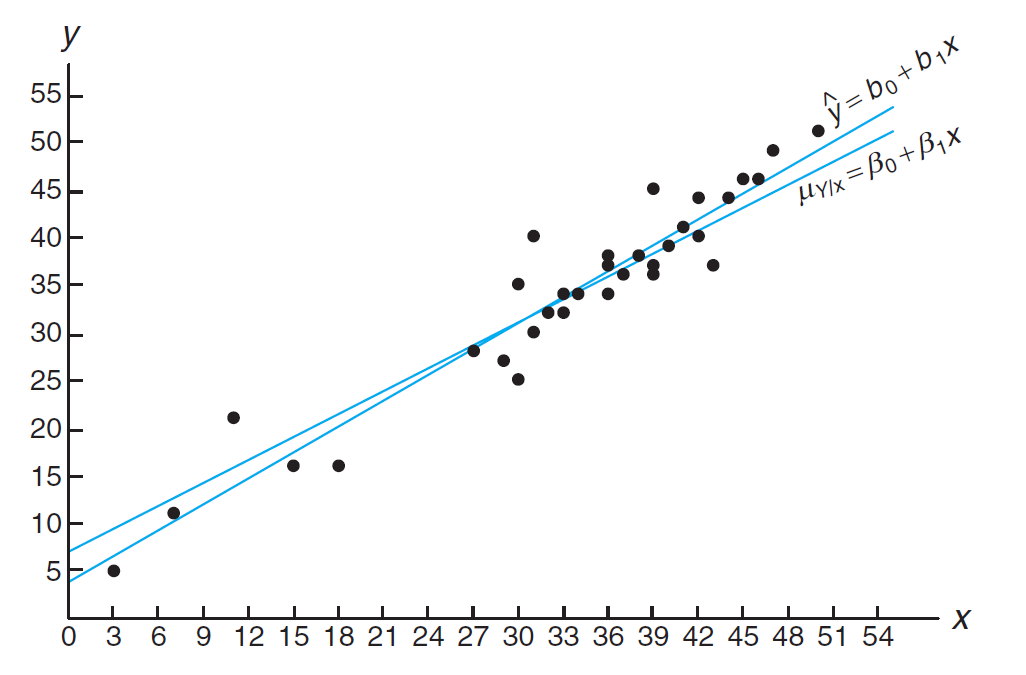
\includegraphics[height=0.7\textheight]{./lr2}
\caption{}
\label{fig:lr2}
\end{figure}

}


\frame{
\frametitle{}
\begin{itemize}
\item Relation with respect of the ''true'' regression line.
\begin{figure}
\centering
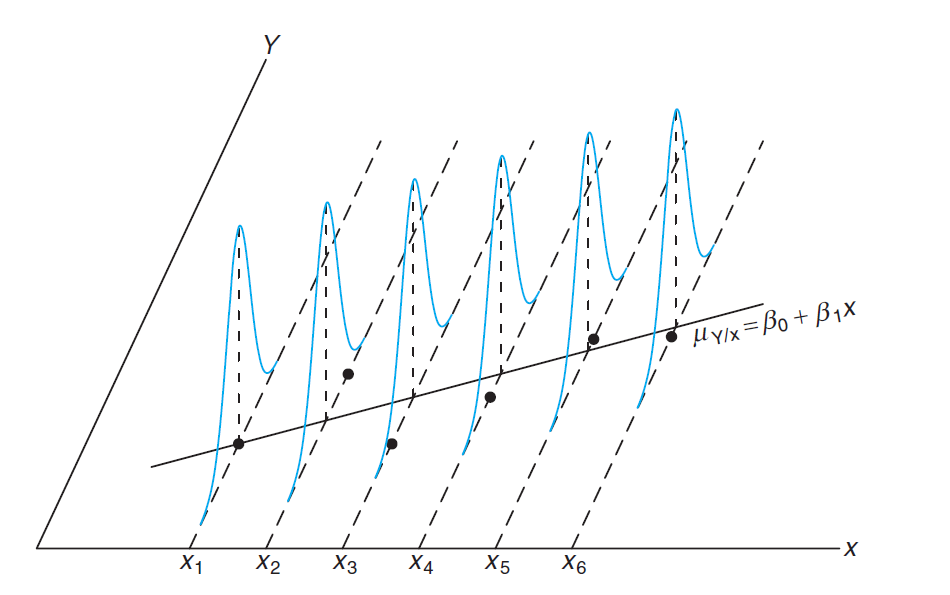
\includegraphics[height=0.7\textheight]{./lr3}
\caption{Individual observations around the true regression}
\label{fig:lr3}
\end{figure}
\end{itemize}
}



\frame{
\frametitle{Residual}
\begin{itemize}
\item Error in fit: Given a set of regression data $\{(x_i,y_i):i=1,2,\dots, n\}$ and a fitted model $\hat{y}= b_0 + b_1 x$, the $i$-th residual, $e_i$, is given by $$e_i= y_i - \hat{y}_i, i=1,2,\dots,n$$
\item $e_i$ is observable
\item $\epsilon_i$ is not observable
\end{itemize}
}

\frame{
\frametitle{Residual}
\begin{figure}
\centering
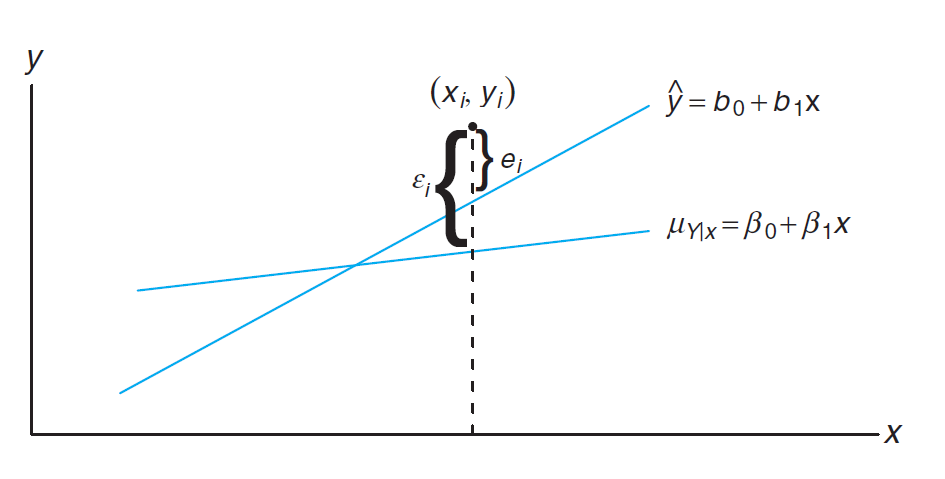
\includegraphics[height=0.7\textheight]{./lr4}
\caption{Comparing $\epsilon_i$ with the residual $e_i$}
\label{fig:lr4}
\end{figure}
}



\frame{
\frametitle{Least Squares}
\begin{itemize}
\item We shall find $b_0$ and $b_1$ so that the sum of the squares of the residuals should be minimum.
\item Sum of squares of the error
\begin{center}
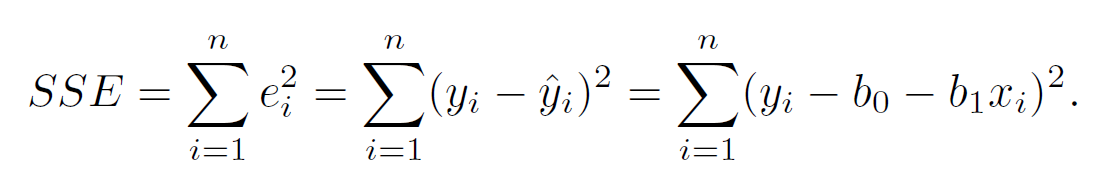
\includegraphics[height=0.18\textheight]{./lr5}
\end{center}
\end{itemize}
}


\frame{
\frametitle{Least Squares}
\begin{itemize}
\item The method for estimating the parameters is called \textbf{least squares}.
\begin{center}
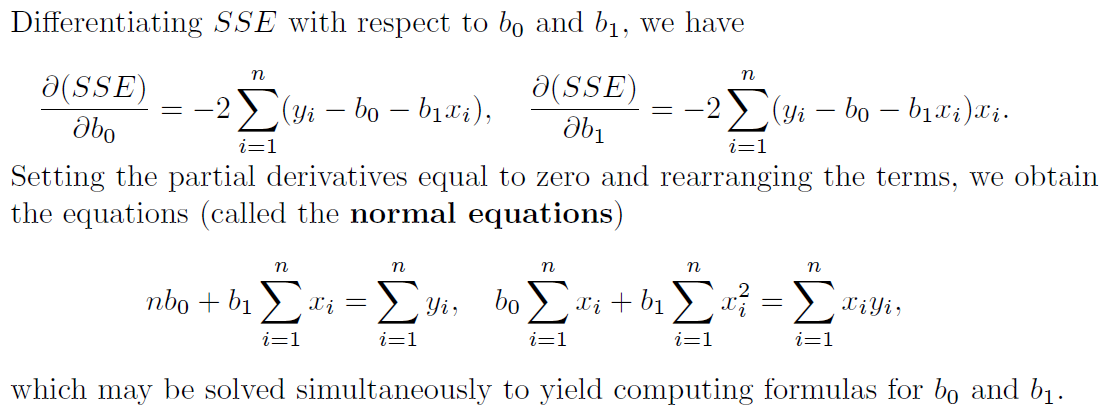
\includegraphics[height=0.6\textheight]{./lr6}
\end{center}
\end{itemize}
}


\frame{
\frametitle{Least Squares}
\begin{itemize}
\item Parameters:
\begin{center}
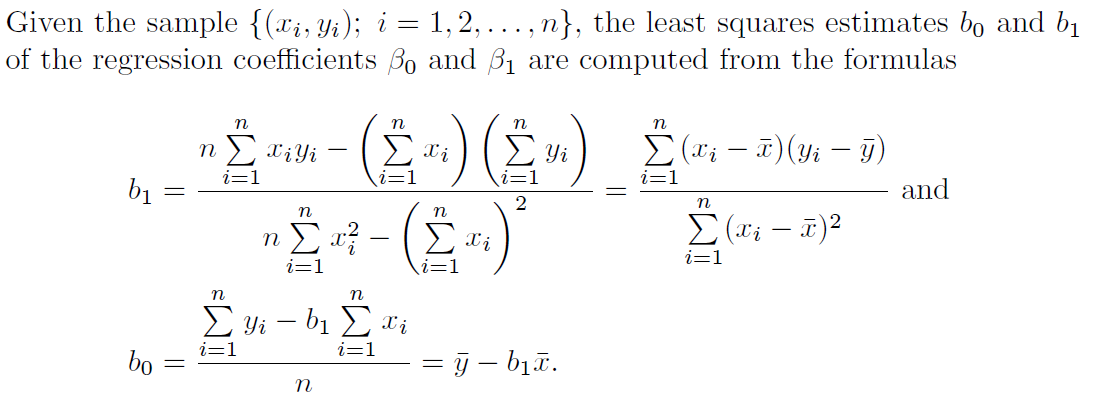
\includegraphics[height=0.6\textheight]{./lr7}
\end{center}
\end{itemize}
}


\frame{
\frametitle{Excercise}
\begin{itemize}
\item \textbf{Ejercicio 11.1,} Walpole, R. E., Myers, R. H., Myers, S. L., \& Ye, K. Probability and statistics for engineers and scientists (9th Ed). New York: Macmillan.
\end{itemize}
\centering
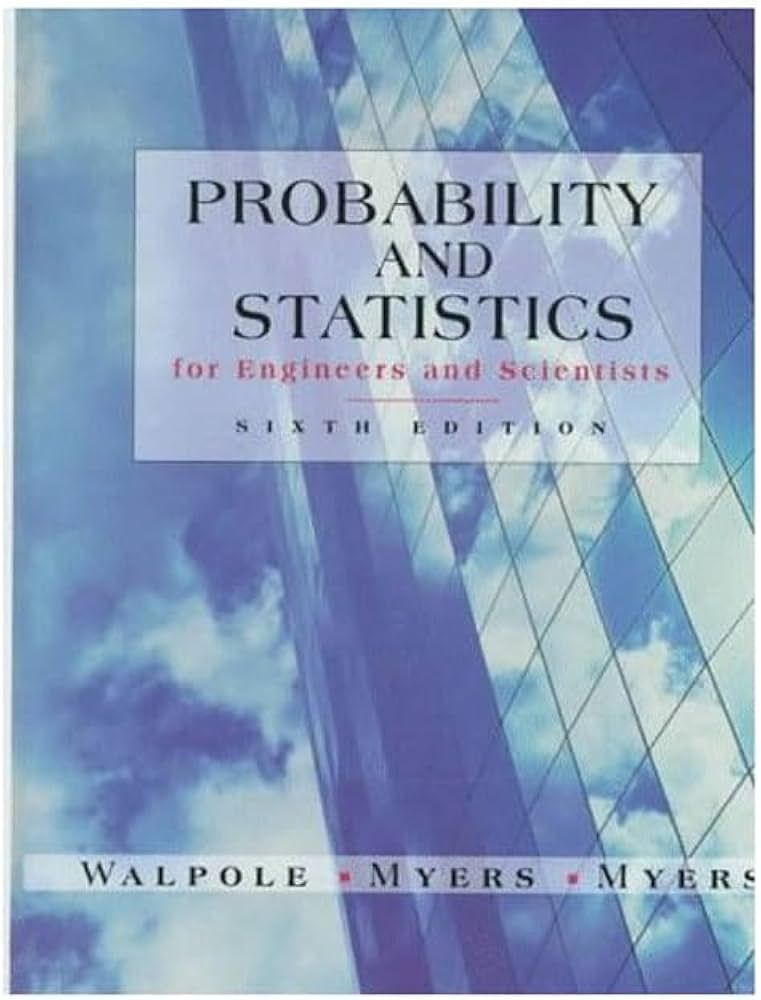
\includegraphics[height=0.4\textheight]{./walpole}
}



\end{document}